\section{ロボットへの応用のためのセンサセットの作成}
\label{chap:app_hand}

\subsection{ハードウェア構成}
\label{sec:hard_content}
ロボットの把持応用のためにロボットのエンドグリッパの上にマイクとスピーカを載せたセンサセットを作成した。ハードウェアの構成について、説明していく。

\begin{table}[h]
    \centering
    \caption{Hard ware consitution}
    \vspace{1zh}
    \begin{tabular}{l||l} \hline
         & Name \\ \hline\hline
        Microphone & Matric Criator \\
        Mirco Computer & Raspberry Pi 3B+ \\
        Speaker & FPS Speaker Unit 0202 \\
        End Effector & EZ Griiper \\ \hline
    \end{tabular}
    \label{tab:hand_hard_content}
\end{table}

\begin{figure}[hb]
  \begin{center}
  \vspace{1zh}
    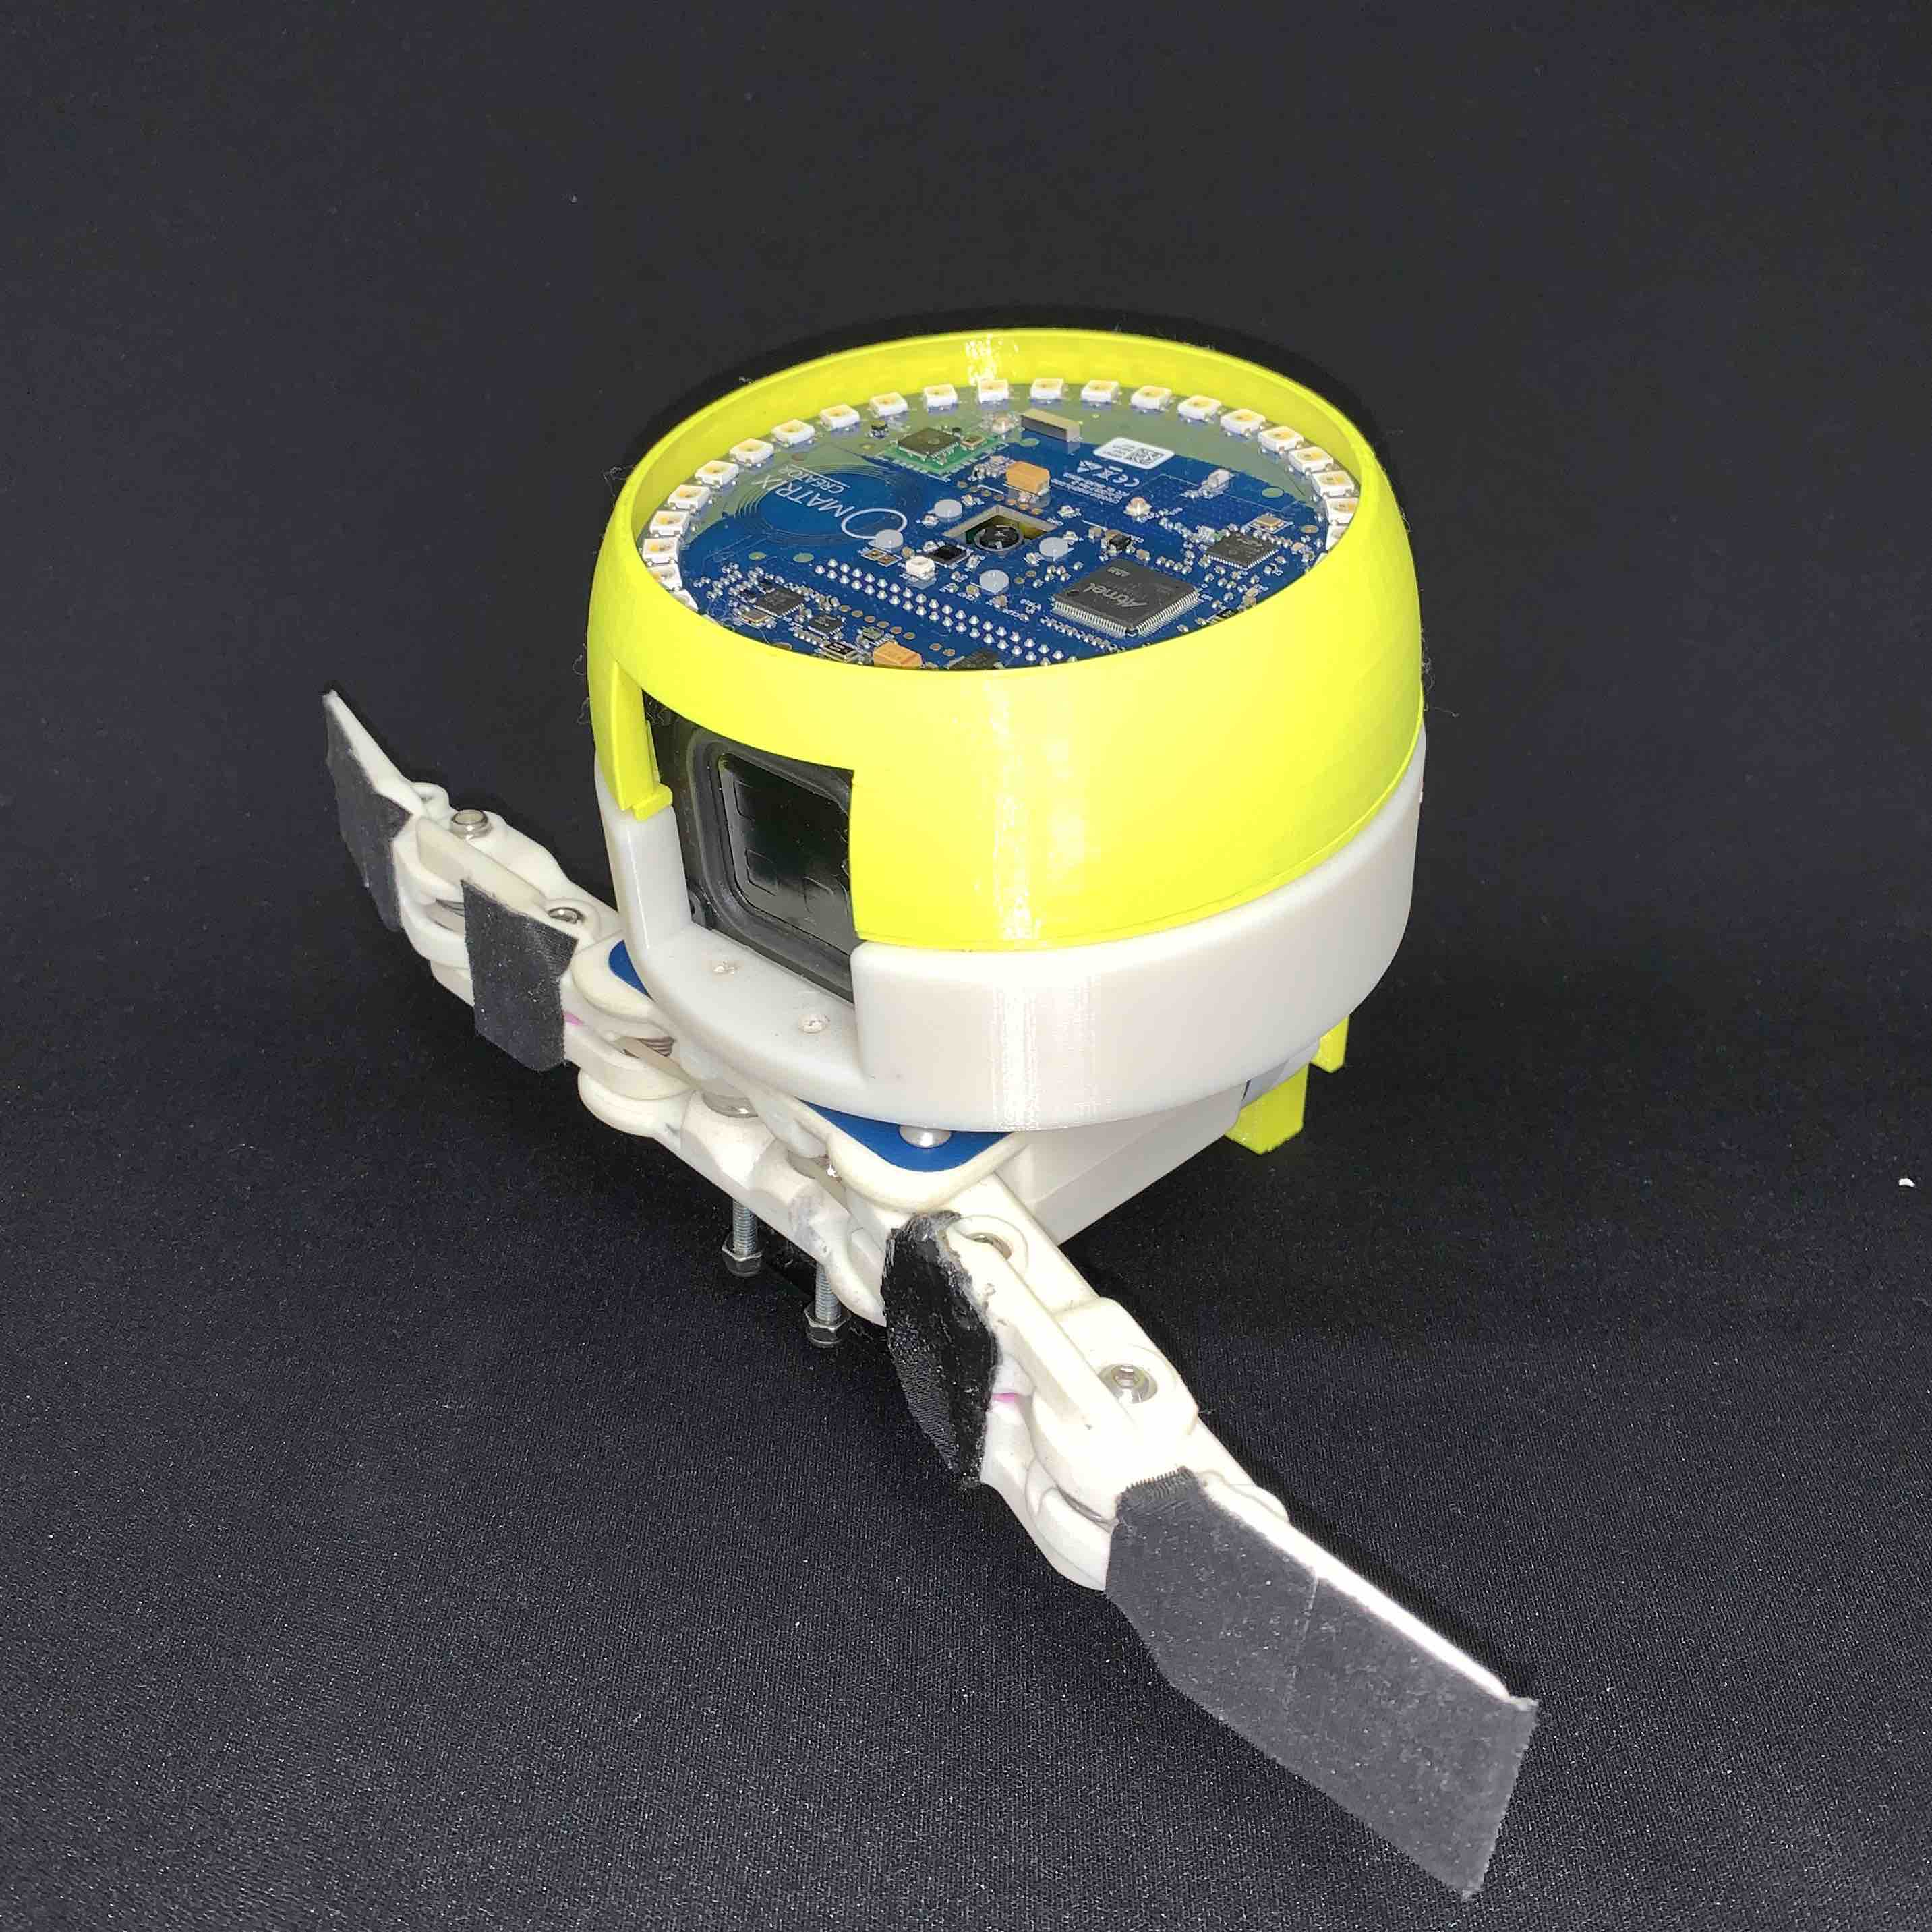
\includegraphics[width=\linewidth]{images/5_sensor_st.jpg}   
  \end{center}
  \caption{Hard ware set}
  \label{fig:hand_hard_image}
\end{figure}

\clearpage

それぞれの使用機器について詳細を説明する。
\subsubsection{Microphone}
MATRIX社のMATRIX Creatorを使用している。特徴としては、8個のマイクロホンアレイを搭載している。さらに、Respeaker Microphone arrayに比べて、マイク間距離が長い。そのため、Beamgformingを使用する際に空間分解能と精度が向上する。さらに、Matrix CreatorはRaspberry Piを使い制御が可能であるため、センサセットとして運用が簡単である。

\begin{figure}[tb]
  \begin{center}
  \vspace{1zh}
    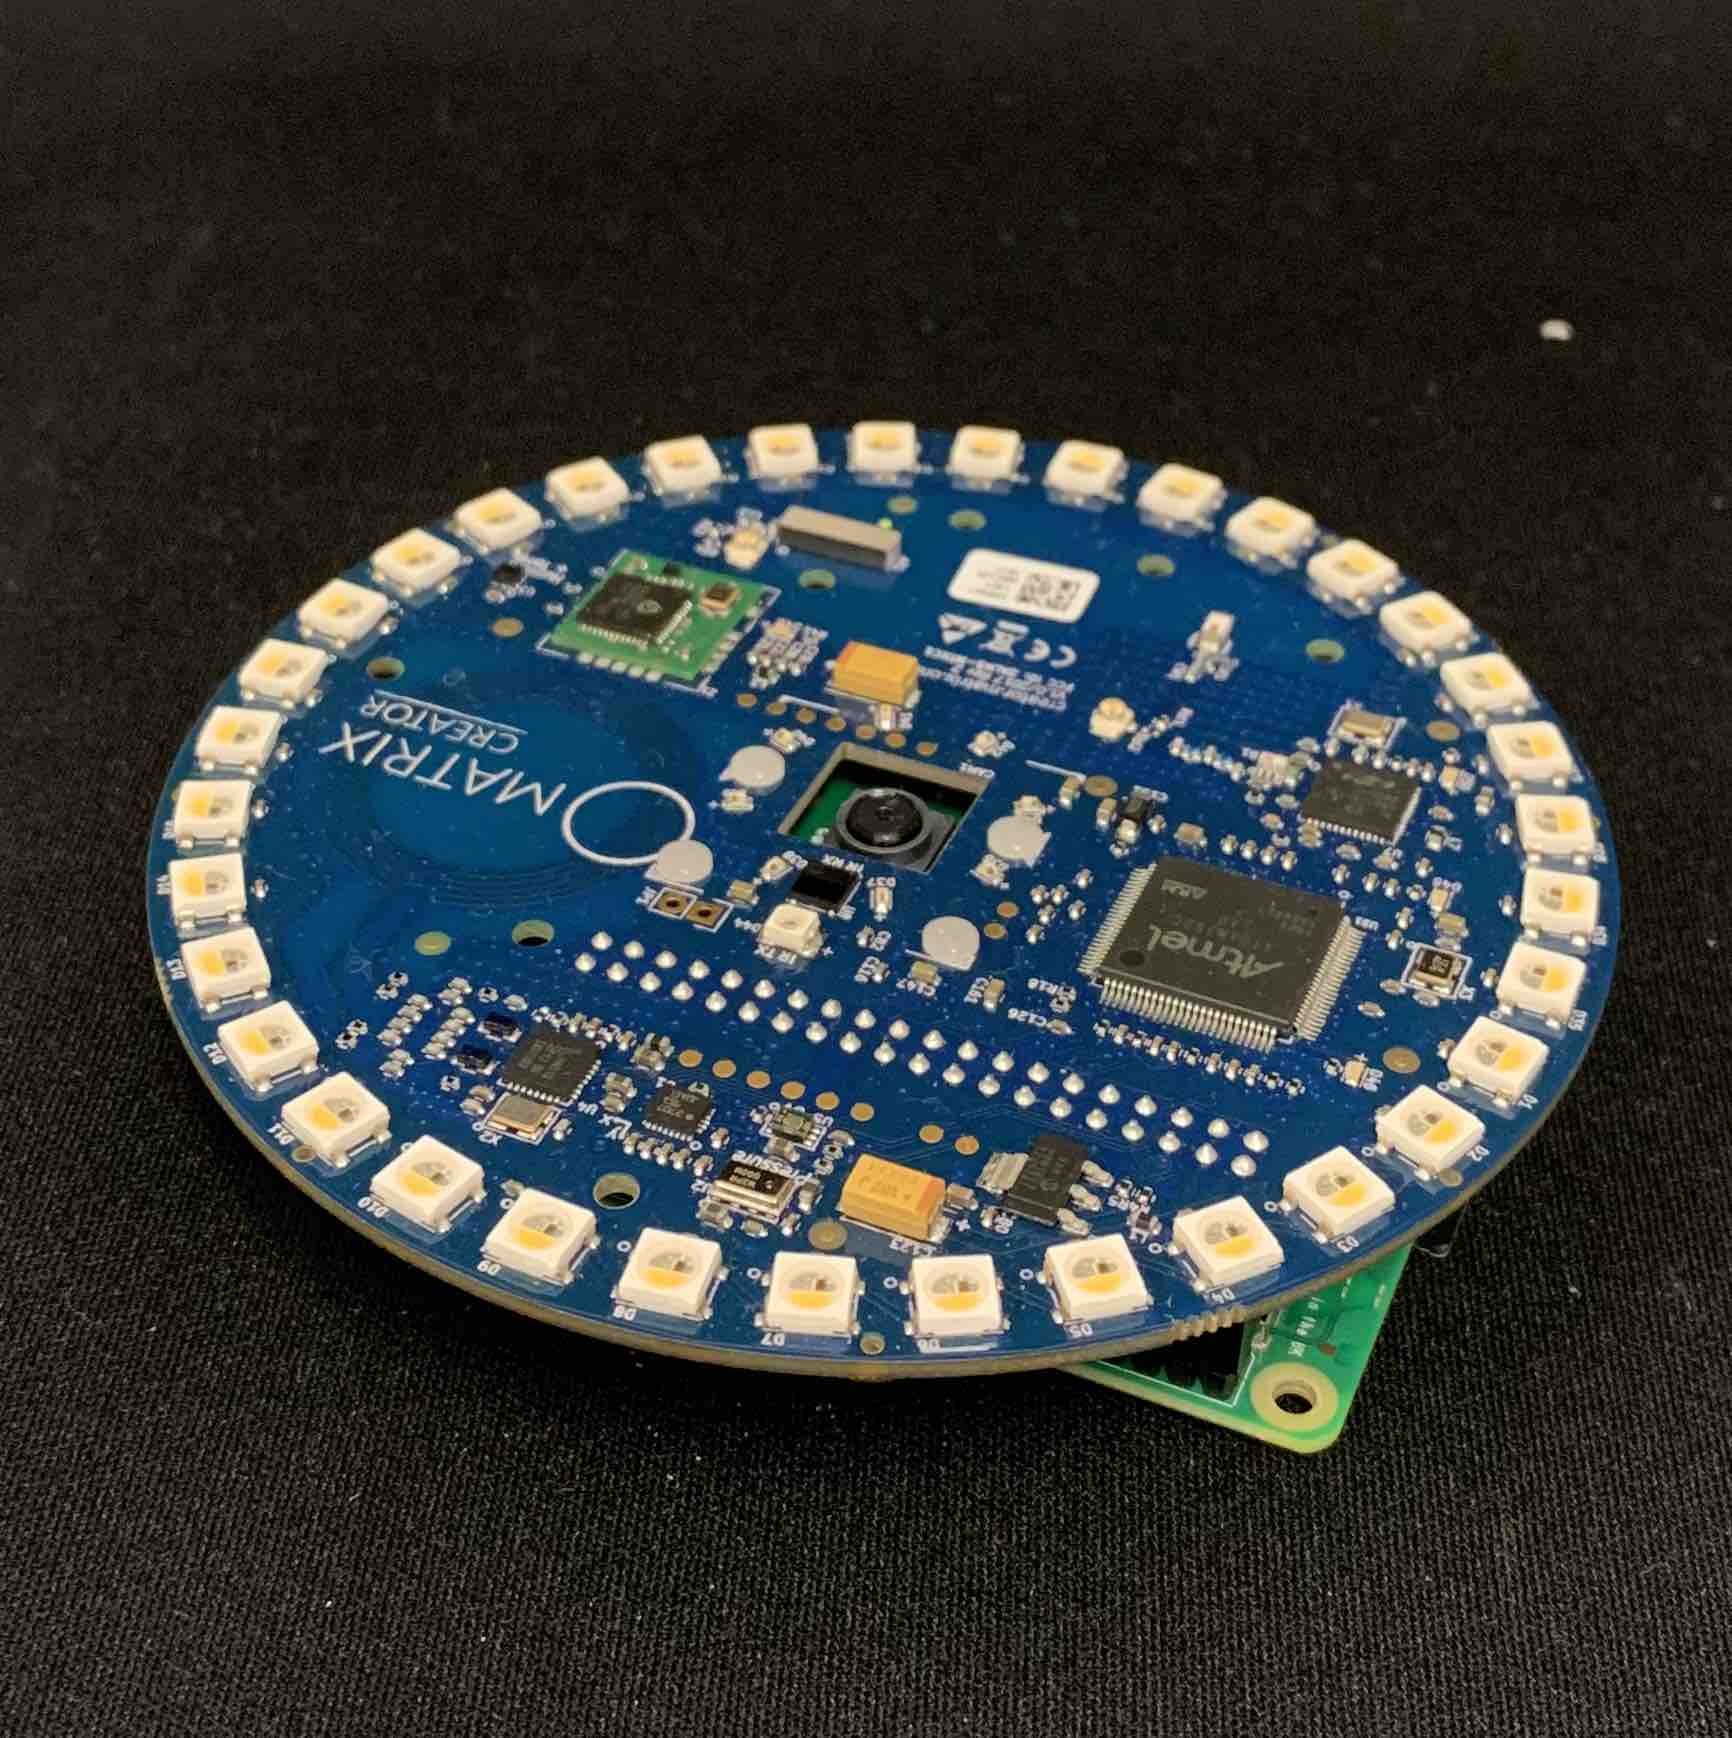
\includegraphics[width=0.7\linewidth]{images/5_matrix_creator.jpg}   
  \end{center}
  \caption{Matrix Creator}
  \label{fig:hand_hard_matrix}
\end{figure}

\subsubsection{Speaker}
FPS社のフラットスピーカユニット0202を使用している。特徴としては平面波スピーカであり、さらに、スピーカの大きさも一番小さい種類を用いている。欠点としては、一般的な球面波スピーカよりかは指向性を持つが、平面波スピーカの中では、指向性が弱いという点である。

\begin{figure}[tb]
  \begin{center}
  \vspace{1zh}
    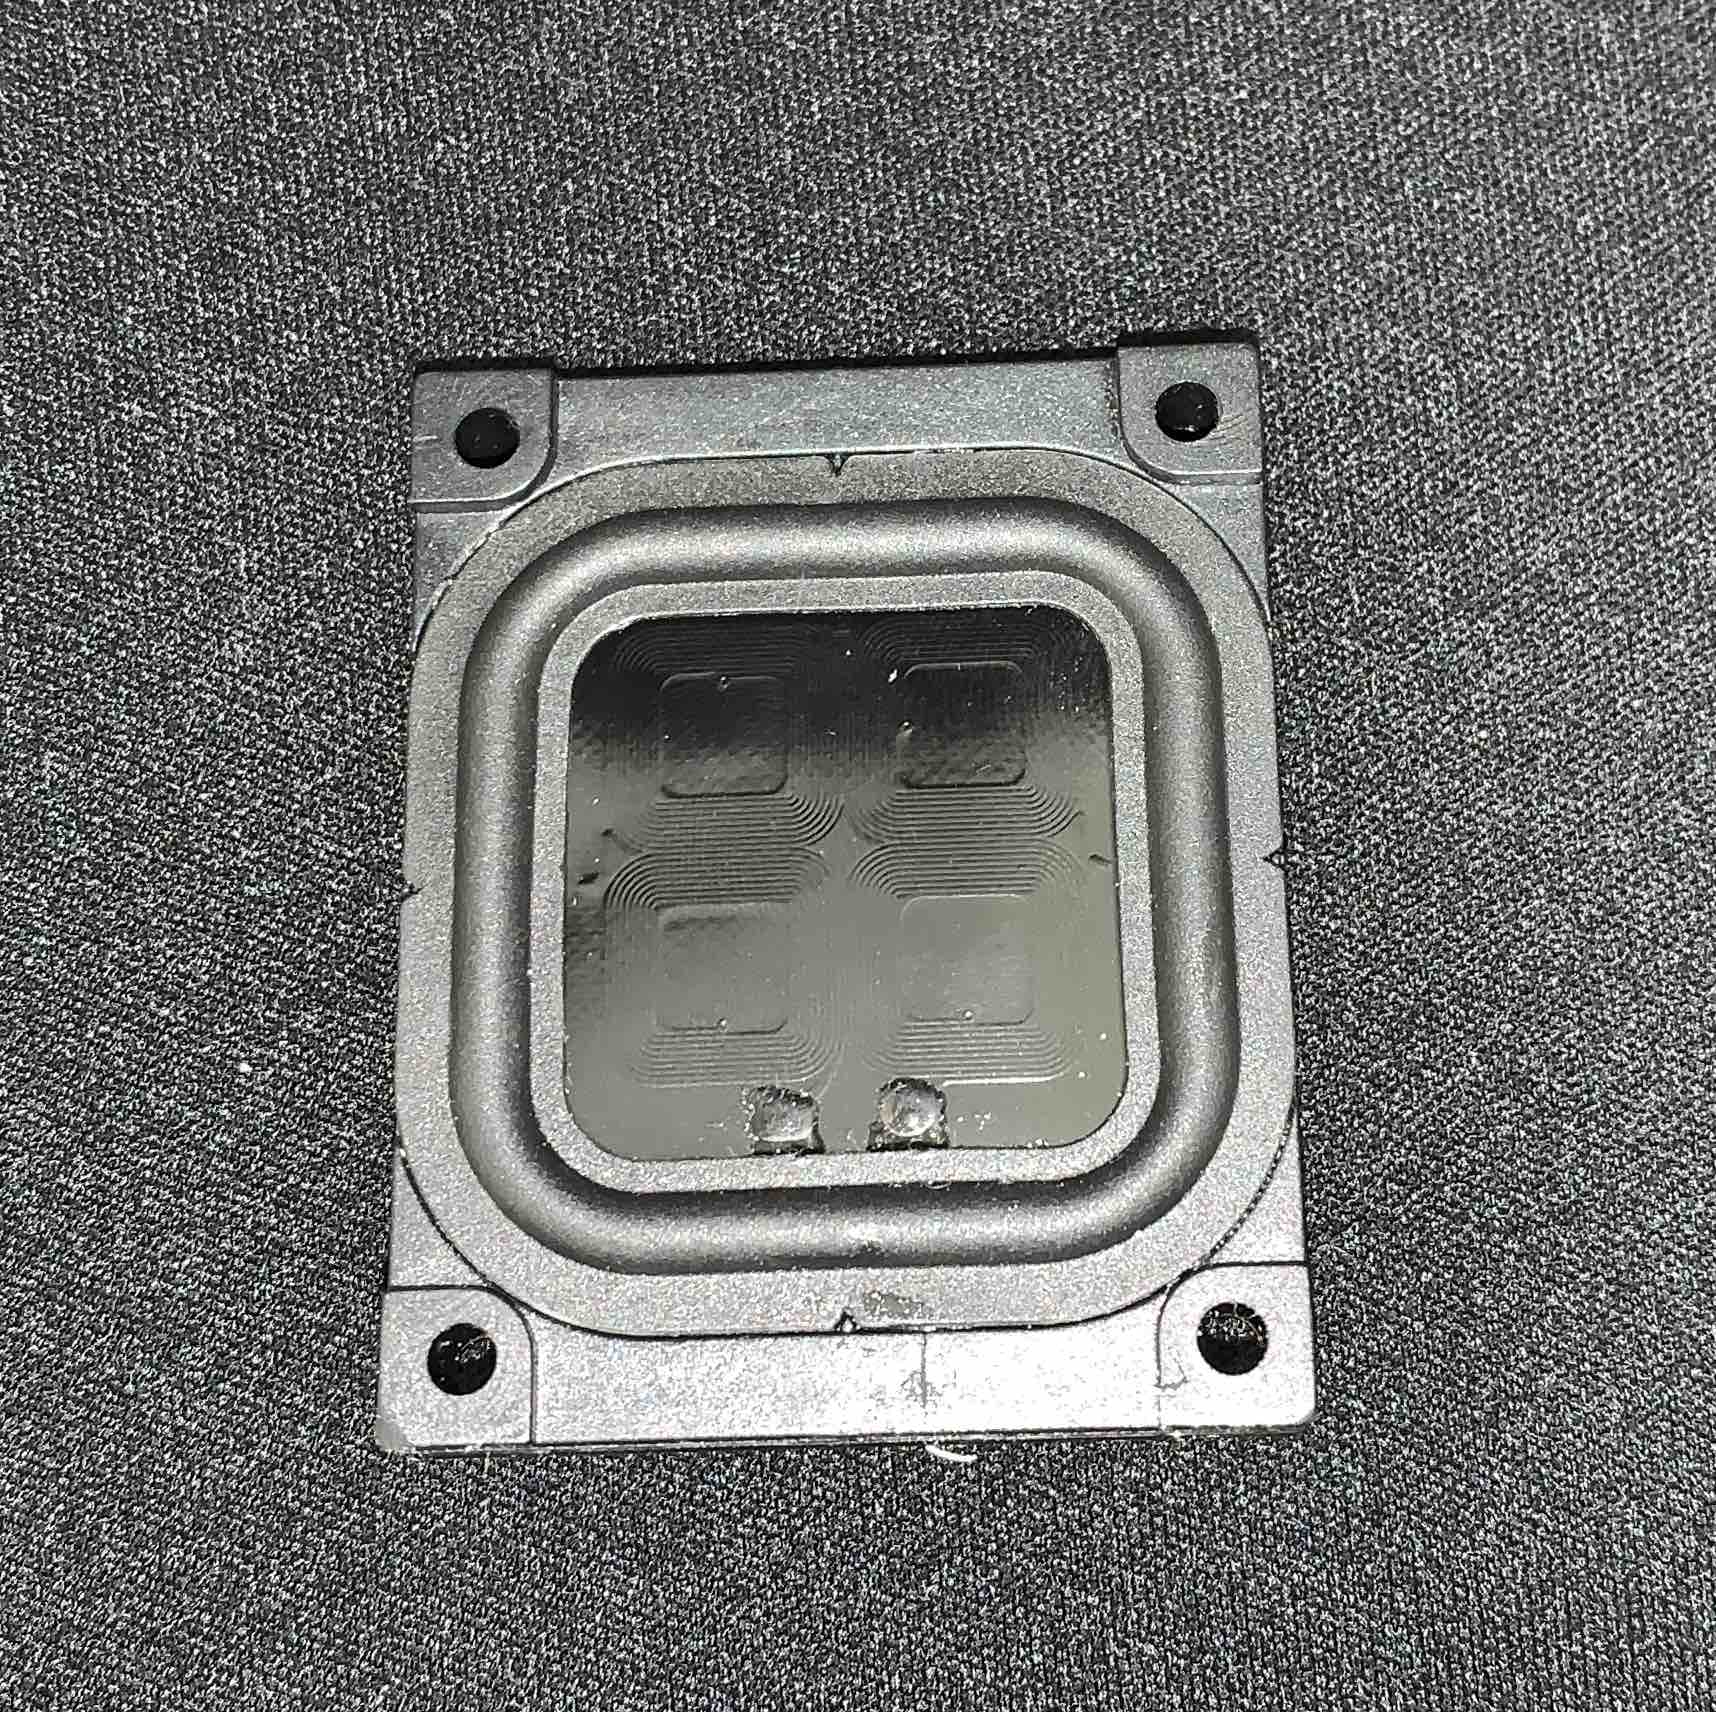
\includegraphics[width=0.7\linewidth]{images/5_fps0202.jpg}   
  \end{center}
  \caption{FPS Speaker 0202}
  \label{fig:hand_hard_fps}
\end{figure}


\subsection{ソフトウェア構成}
\label{sec:soft_system}
ソフトウェアのフローチャートを\figref{hand_soft_flow}に示す。
スピーカ、マイクの制御はRaspberry Pi 3B+を用いて行う。また、今回はセンサセットのみの評価を行うため、エンドエフェクタの制御は含んでいない。

マイクでの入力音の処理は\secref{make_data_set}のデータセット作成方法と同様の処理を行い、1000 [Hz] - 2000[Hz]の平均0分散1で正規化した周波数領域のデータに変換する。このデータを入力として、SVRで作成したモデルで面の方位角の推定を行う。
このときの、SVRのモデルはこれまで用いていたSVRのモデルではなく、センサセットを用いて集めたデータセットで学習を行ったSVRモデルを使用している。今回、前回のモデルが使用できない理由として、考えられるものはマイク、スピーカが完全に別のものになったことが考えられる。マイクやスピーカの周波数特性に対して影響があると考え、新たなモデルを作成した。

\begin{figure}[tb]
  \begin{center}
  \vspace{1zh}
    
\includegraphics[width=0.7\linewidth]{images/fig_sample.png}   
  \end{center}
  \caption{Flow Chart}
  \label{fig:hand_soft_flow}
\end{figure}

\clearpage

\subsection{実験方法}
\label{sec:hand_exp_env}
実験方法は\chapref{exp_azimuth_angle}と同様に行う。

そのため、実験環境も\chapref{exp_azimuth_angle}、\chapref{application_experiment}同様に奈良先端大において実験を行った。
本実験の目的は以下の2点である。

\begin{itemize}
    \item 方位角推定ができるか?
    \item 複数面の認識ができるか?
\end{itemize}

以上の2点について、実験を行う。その様子を\figref{hand_exp_env}に示す。
対象物体としては、\chapref{exp_azimuth_angle}において、もっとも精度がでた鏡??を用いる。


\begin{figure}[tb]
    \centering
    \subfigure[Solo Plate]{
\includegraphics[width=0.7\linewidth]{images/fig_sample.png}}
    \label{fig:hand_exp_1plate}
    \subfigure[Multi Plate]{
\includegraphics[width=0.7\linewidth]{images/fig_sample.png}}
    \label{fig:hand_exp_2plate}
    \caption{Experiment Environment}
    \label{fig:hand_exp_env}
\end{figure}

\clearpage

\subsection{方位角推定による評価}
\label{sec:hand_result}
結果を\figref{hand_result}に示す。また、このときのそれぞれの決定係数、二乗平均平方誤差を\tabref{hand_result_svr}に示す。

\begin{figure}[tb]
    \centering
    \subfigure[Solo Plate]{
\includegraphics[width=0.45\linewidth]{images/fig_sample.png}}
    \label{fig:hand_result_1plate}
    \subfigure[Multi Plate]{
\includegraphics[width=0.45\linewidth]{images/fig_sample.png}}
    \label{fig:hand_result_2plate}
    \caption{Result}
    \label{fig:hand_result}
\end{figure}

\begin{table}[tb]
\caption{Result of SVR}    
\vspace{1zh}
\centering
  \begin{tabular}{|l|p{6em}|p{6em}|} \hline
    Data & $\mathrm{R}^2$ & RMSE [deg] \\ \hline\hline 
    Solo & ?? &  ?? \\ \hline 
    Multi & ?? &  ?? \\ \hline
  \end{tabular}
  \label{tab:hand_result_svr}
\end{table}

\subsection{考察}
\label{sec:hand_disscusion}
結果として... 

ロボットの動作に関しては今回は含めていない。ロボットを動作させた場合、ロボットによる雑音により認識できないと考えたためである。この雑音処理については今後の展望としていきたい。

\newpage